\documentclass[12pt,authoryear]{elsarticle}
%\documentclass[12pt]{article}
% \usepackage[margin=1in]{geometry}
% \usepackage[margin=0.5in]{caption}
\usepackage{amsmath}
\usepackage{amssymb}
%\usepackage{natbib}
\usepackage{amsthm}
\usepackage{hyperref}
%\usepackage{graphicx}
\usepackage{xcolor}
\usepackage{booktabs}
\usepackage{soul}
\usepackage[ruled]{algorithm2e}
\usepackage{bm}
\usepackage{subcaption}
\usepackage{wrapfig}
% \usepackage{setspace}
% \linespread{1.8}
\usepackage{anysize}
\marginsize{1in}{1in}{1in}{1in}

\newtheorem{prop}{Proposition}
\DeclareMathOperator{\tr}{Tr}
\DeclareMathOperator*{\argmin}{arg\,min}
\DeclareMathOperator*{\argmax}{arg\,max}
\newcommand{\bigmid}{\,\middle\vert\,}
% \newcommand{\bruno}[1]{\textcolor{blue}{#1}} % Bruno Sanso edits - blue
% \newcommand{\makenote}[1]{\textcolor{red}{#1}} % Peter edits - red


\newcommand{\findcite}{\textcolor{red}{[Find Citation]}}
\newcommand{\needcite}{\findcite}
\newcommand{\Chi}{\mbox{\Large$\chi$}}
\newcommand{\norm}[1]{\left\lVert #1 \right\rVert}
\newcommand{\inorm}[1]{\norm{#1}_{\infty}}
\newcommand{\pnorm}[2]{\norm{#1}_{#2}}
\newcommand{\prob}[1]{\text{Pr}\left[#1\right]}
\newcommand{\expect}[1]{\text{E}\left[#1\right]}

\SetAlCapNameFnt{\footnotesize}
\SetAlCapFnt{\footnotesize}
\SetAlCapSty{}




\begin{document}

\begin{frontmatter}
    %\title{Inference for multivariate peaks over threshold models}
    \title{Bayesian non-parametric inference for multivariate peaks-over-threshold models}
    \author{Peter Trubey\corref{cor1}}
    \ead{ptrubey@ucsc.edu}

    \author{Bruno Sans\'o}
    \ead{bruno@soe.ucsc.edu}
    \address{Department of Statistics, University of California, Santa Cruz,  USA}
    \cortext[cor1]{Corresponding author}
    
    \begin{abstract}
        
We consider a constructive definition of the multivariate Pareto that factorizes the 
random vector into a radial component and an independent angular component; the former
following a univariate Pareto distribution, and the latter defined on the surface of the 
positive orthant of the unit hypercube.  In this paper, we  propose a method for
inferring the distribution of the angular component.  We identify its support 
as the limit of the positive orthants of the unit $p$--norm spheres.
To this effect, we introduce a projected gamma family of
distributions defined as the projection of a vector of independent gamma random variables
onto the $p$--norm sphere.  This family serves as a building block for a flexible family
of distributions obtained as a Dirichlet process mixture of projected gammas.  For 
model assessment and comparison, we discuss model scoring methods appropriate 
to distributions on the unit hypercube.  In particular, working with the energy score
criterion, we develop a kernel metric appropriate to the hypercube that produces a 
proper scoring rule.  We then present a simulation study to compare 
different modeling choices using the proposed scoring rules.  Finally we apply our 
approach to describe the dependence structure of the extreme values of the magnitude 
of the integrated vapor  transport (IVT), a variable that describes the rate of flow 
of moisture in the atmosphere  along the coast of California for the years of 1979 
through 2020.  We find a clear but heterogeneous geographical dependence.
%We present the results 
%of this analysis to describe the dependence structure of extreme events in IVT using 
%pairwise extremal dependence coefficients---a summary measure of jointly extreme behavior.
%We also present conditional survival curves---the survival function for some dimensions
%conditional on other dimensions.

% EOF
    \end{abstract}

    \begin{keyword}
        Multivariate extremes \sep Peak over threshold models \sep
        Bayesian non-parametric models \sep Dirichlet process mixtures
    \end{keyword}
\end{frontmatter}

%--------content

\section{Introduction}

The statistical analysis of extreme values focuses on inference for
    rare events that correspond to the tails of probability distributions.
    As such, it is a key ingredient in the risk assessment of
    phenomena that can have strong societal impacts like floods, heat waves,
    high concentration of pollutants, crashes in the financial markets,
    among others. The fundamental challenge of extreme value theory (EVT) is
    to use information, collected over limited periods of time, to
    extrapolate to long time horizons. This sets EVT apart from most of
    statistical inference, where the focus is on the bulk of the
    distribution. Extrapolation to the tails of the distributions is
    possible thanks to theoretical results that give asymptotic descriptions
    of the probability distributions of extreme values. 

Inferential methods for the extreme values of univariate observations
    are well established and software is widely available 
    \cite[see, for example,][]{coles2001}. For variables in one dimension the 
    application of EVT methods considers the asymptotic distribution of either the 
    maxima calculated for regular blocks of data, or the values that exceed a 
    certain threshold. The former leads to a Generalized Extreme Value (GEV) 
    distribution, that depends on three parameters. The latter leads to a Generalized 
    Pareto (GP) distribution, that depends on a shape and a scale parameter. 
    Likelihood-based approaches to inference can be readily implemented in both cases.
    In the multivariate case the GEV theory is well developed 
    \citep[see, for example][]{dehaan2006}, but the inferential problem is more 
    complicated, as there is no parametric representation of the GEV. This problem
    is inherited by the peaks over threshold (PoT) approach and compounded by the 
    fact that there is no unique definition of an exceedance of a multivariate 
    threshold, as there is an obvious dependence on the norm that is used to measure 
    the size of a vector. 

During the last decade or so, much work has been done in the exploration of the 
    definition and properties of an appropriate generalization of the univariate 
    GP distribution to a multivariate setting.  To mention some of the papers on 
    the topic, the work of \citep{rootzen2006} defines the generalized Pareto 
    distribution, with further analysis on these classes of distributions 
    presented in \cite{falk2008} and \cite{michel2008}.  A recent review of the 
    state of the art in multivariate peaks over threshold modelling using 
    generalized Pareto is provided in \cite{rootzen2018} while \cite{RoSeWa2018a} 
    provides insight on the theoretical properties of possible parametrizations. 
    These are use in \cite{KiRoSeWa2019} for likelihood-based models for PoT 
    estimation. A frequently used method for describing the dependence in 
    multivariate distributions is to use a copula. \cite{renard2007}, and 
    \cite{falk2019} provide successful  examples of this approach in an EVT 
    framework. \cite{ferreira2014} presents a constructive definition of the 
    Pareto process, that generalizes the GP to an infinite dimensional setting. It 
    consists of decomposing the process into independent radial and angular 
    components. Such an approach can be used in the finite dimensional case, where 
    the angular component contains the information pertaining to the dependence 
    structure of the random vector. Based on this definition, we present a novel 
    approach for modelling  the angular component with families of distributions 
    that provide flexibility and can be applied in a moderately large dimensional 
    setting.  Our focus on the angular measure is similar to that in \cite{boldi2007},
    \cite{SaNa2014} and \cite{HaCaCh2017}, that consider Bayesian non-parametric 
    approaches. Yet, our approach differs in that it is established in the 
    peaks-over-threshold regime, and avoids the problem of dealing with the so 
    called moment constraint by considering a constructive definition of the 
    multivariate GP, based on the infinity norm.  Further, the 
  
The reminder of this paper is outlined as follows. 
    Section~\ref{sec:multivariatepot} comprises a brief review of multivariate PoT, 
      detailing the separation of the radial measure from the angular measure.
    Section~\ref{sec:methodology} details our approach for estimating the angular 
      measure, based on projecting an arbitrary distribution supported in ${\mathbb R}_+^d$ 
      onto unit hyper-spheres defined for $p$-norms. 
    Section~\ref{sec:evaluation} develops criteria for model selection in the support 
      of the angular measure.  
    Section~\ref{sec:results} explores the efficacy of the proposed approach on a set 
      of simulated data, and, acknowledging the relevance of extreme value theory to 
      climatological events~\citep{jentsch2007,vousdoukas2018,li2019}, estimates the 
      extremal dependence structure for a measure of water vapor flow in the atmosphere, 
      used for identifying atmospheric rivers.  
    Finally, Section~\ref{sec:conclusion} presents our conclusions and discussion.

Throughout the paper, we adopt the operators $\wedge$ to denote minima, and 
    the $\vee$ to denote maxima.  Thus $\wedge_i s_i = \min_i s_i$, and 
    $\vee_i s_i = \max_i s_i$.  These operators can also be applied component-wise 
    between vectors, such as $\bm{a}\wedge\bm{b} = (a_1\wedge b_1, a_2\wedge b_2,\ldots)$.  
    We use uppercase to indicate random variables, lowercase to indicate points, and
    bold-face to indicate vectors or matrices thereof.
  
\section{A multivariate PoT model\label{sec:multivariatepot}}
To develop a multivariate PoT model for extreme values consider a 
    $d$-dimensional random vector $\bm{W} = (W_1, \ldots ,W_d)$ with
    cumulative distribution $F$. Following \cite{RoSeWa2018a}, assume 
    that there exists sequences of vectors $\bm{a}_n$ and $\bm{b}_n$,
    and a $d$-variate distribution $G$ such that 
    $\lim_{n\rightarrow\infty} F^n(\bm{a}_n \bm{w} + \bm{b}_n) = 
    G(\bm{w})$. $G$ is a $d$-variate generalized extreme value 
    distribution. It follows that
    \begin{equation*}
        \begin{aligned}
        \lim\limits_{n\rightarrow\infty} &\prob{\bm{a}^{-1}_n (\bm{W} - \bm{b}_n) 
      \leq \bm{w} \mid \bm{W} \not\leq \bm{b}_n)} \\ 
        &\hspace{0.5cm}= \frac{\log G(\bm{w} \wedge \bm{0}) 
        - \log G(\bm{w}) }{\log G(\bm{0})} = H(\bm{w}).
        \end{aligned}
    \end{equation*}
    $H$ a multivariate Pareto distribution, and corresponds to the joint
    distribution conditional on exceeding a multivariate threshold. In addition to
    a copula function, $H$ depends on two $d$-dimensional vectors of 
    parameters that we denote as $\bm{\xi}$ for the shapes and $\bm{\sigma}$ 
    for the scales. \cite{RoSeWa2018a} provide a number of stochastic 
    representations for $H$.  In particular, denote as $Z$ a
    random variable with distribution $H$ where $\bm{\xi}= 1$ and 
    $\bm{\sigma} = 0$.  Then, Remark 1 justifies the representation in 
    \cite{ferreira2014}, giving $\bm{Z} = \bm{V}R$
    where $R$ and $\bm{V}$ are independent. $R = \|\bm{Z}\|_\infty$ is 
    distributed as a standard Pareto random variable, and $\bm{V} = 
    \bm{Z}/\|\bm{Z}\|_\infty$ is a random vector in  
    $\mathbb{S}_{\infty}^{d-1}$, the positive orthant of the 
    unit sphere under $\mathcal{L}_{\infty}$ norm, with distribution $\Phi$. 
    This representation is central to the methods proposed in this paper.
    $R$ and $\bm{V}$ are referred to, respectively, as the {\em radial} 
    and {\em angular} components of $H$. The angular measure controls 
    the dependence  structure of $\bm{Z}$  in the tails. In view of 
    this, to obtain a  PoT model we seek a flexible model for the 
    distribution of $\bm{V} \in {\mathbb S}_{\infty}^{d-1}$.

The approach considered in \cite{rootzen2018} focuses on the limiting
    conditional distribution $H$. An alternative approach consists of assuming
    that regular variation \cite[see, for example,][]{resnick2008extreme} holds 
    for the limiting distribution of $\bm{W}$, implying
    \[
        \lim\limits_{n\rightarrow\infty} n \prob{n^{-1} \bm{W}\in A} = 
        \mu(A),
    \]
    where $\mu$ is termed the exponent measure. $\mu$ has the homogeneity property
    $\mu(tA) = t^{-1}\mu(A)$. Letting $\rho = \|W\|_p, p>0$ 
    and $\bm{\theta} = \bm{W}/\rho$, define  $\Psi(B) = \mu(\{\bm{w} : \rho>1, 
    \bm{\theta} \in B\})$, which is referred to as the angular measure. After 
    some manipulations, we obtain that
    \begin{equation}
    \label{exponent-mu}
        \lim\limits_{r\rightarrow\infty} 
        \text{Pr}\left[\bm{\theta}\in A \rvert \rho>r\right] = 
            \frac{\Psi(A)}{\Psi({\mathbb S}_p^{d-1})} .
    \end{equation}
    Thus, a model for the exponent measure induces a model for the limiting distribution
    conditional on the observations being above a threshold defined with respect
    to their $p$-norm. The constraint that all marginals of $\mu$ correspond to a
    standard Pareto distribution leads to the so called moment constraints on $\Psi$. 
    Inference for the limiting distribution of the exceedances
    needs to account for the normalizing constant in Equation \ref{exponent-mu}, as well
    the moment constraints. In addition, the moment constraints can impose unrealistic
    symmetries in the data distribution.

% EOF


\section{Estimation of the angular measure\label{sec:methodology}}

Our approach to estimating the PoT distribution considers two steps: First we 
    estimate the shape and scale parameters for the
    multivariate Pareto distribution, using the univariate marginals; Then 
    we focus on the dependence structure in extreme regions by proposing a 
    flexible model for the distribution of $\bm{V}$. Consider a collection of 
    observations  $\bm{w}_i \in {\mathbb R}^d, i = 1, \ldots, n$ that exhibit 
    extreme behavior.  We \bruno{start by setting a large threshold 
    $b_{t,\ell}$ for the  $\ell$-th marginal, $\ell = 1, \ldots,d$. Then, the 
    distribution of the observations for the $\ell$-th component, 
    conditional on exceeding the threshold, can be 
    approximated as $1 - (1 + \xi_\ell   (w_{i\ell} - b_{t,\ell})/\sigma_\ell)_+^
    {1/\xi_ell}$, where $(\cdot)_+$ indicates the positive part function.  We 
    proceed by setting a} threshold equal to the empirical $(1-1/t)$-quantile. 
    Thus $b_{t,l}  = \hat{F}^{-1}_{\ell}(1 - 1/t)$. \bruno{We then use the 
    approximate exceedance distribution to estimate $\xi_\ell$ and $\sigma_\ell$,
    for each $\ell$, using likelihood based methods. Then, in order to estimate 
    the angular distribution, we use those estimates to standardize each of 
    the marginals.} The   standardization  yields
    \begin{equation}
            \label{eqn:standardization}
            z_{i\ell} = \left(1 + \xi_{\ell}\frac{w_{i\ell} -
                b_{\ell}}{a_{\ell}}\right)_{+}^{1/\xi_{\ell}}\; .
        \end{equation}
    Note that $z_{i\ell}> 1$ implies that $w_{i\ell} > b_{t,\ell}$, meaning 
    that the observation $\bm{w}_i$ is extreme in the $\ell$-th dimension. 
    Thus, $r_i = \|\bm{z}_i\|_\infty > 1$ implies that at
    least one dimension has an extreme observation, and corresponds 
    to a very extreme observation when $t$ is large. We focus on 
    the observations that are such that $r_i > 1$. These provide a
    sub-sample of $r_i$ and $\bm{v}_i = \bm{z}_i /r_i \in 
    \mathbb{S}_{\infty}^{d-1}$ that is used for  the estimation of 
    $\Phi$ conditional on the sample. We observe that in practice, the choice
    of $\bm{b}$, and the subsequent fitting of $\bm{a}$ and $\bm{\xi}$ induces
    a stochastic element in the spectral distribution that is not accounted for
    in our analysis.  \makenote{phrasing?}

\subsection{Projected gamma family\label{subsec:projgamma}}
To obtain a distribution on 
${\mathbb S}_{p}^{d-1}=\{\bm{s} : \bm{s} \in {\mathbb R}_{+}^{d}, \| \bm{s}\|_{p} = 1\}$ 
we start with a vector in 
$\bm{x} \in {\mathbb R}^d_+$, calculate its $\mathcal{L}_p$-norm  defined as
  \begin{equation*}
    \lVert \bm{x} \rVert_p = 
    \left({\textstyle\sum}_{\ell = 1}^d \lvert s_{\ell}\rvert^p\right)^{\frac{1}{p}},
  \end{equation*}
  and normalize it to obtain $\bm{y} = \bm{x}/\|\bm{x}\|_p \in {\mathbb S}_p^{d-1}$. 
  The absolute and Euclidean norms are obtained for $p=1$ and $p=2$ respectively,
  and the $\mathcal{L}_{\infty}$ norm can be obtained as a limit, 
  \begin{equation*}
    \| \bm{s} \|_{\infty}
      = \lim\limits_{p\to\infty} \| \bm{s} \|
      = \underset{\ell = 1}{\overset{d}{\bigvee}}s_{\ell}.
  \end{equation*}

A natural  distribution to consider in ${\mathbb R}^d_+$ is given by a product of independent
  univariate Gamma distributions. Let
    $\bm{ X} \sim \prod_{\ell = 1}^d\text{Ga}\left(X_{\ell}\mid\alpha_{\ell},\beta_{\ell}\right)$, 
    $\alpha_\ell$ and $\beta_\ell$ are the shape and scale parameters, respectively. 
    For any finite $p$, letting 
   $ y_d = (1 - {\textstyle\sum}_{\ell = 1}^{d-1}y_{\ell}^p)^{1/p}$,
    the transformation
  \begin{equation}
    \label{eqn:pnormt}
    \begin{aligned}
    T(x_1,\ldots,x_d) &= \left(\pnorm{\bm{x}}{p}, \frac{x_1}{\pnorm{\bm{x}}{p}},
                          \ldots , \frac{x_{d-1}}{\pnorm{\bm{x}}{p}}\right) \\
                        &= (r,y_1,\ldots,y_{d-1})
    \end{aligned}
  \end{equation}
  is invertible with
  \begin{equation}
    \label{eqn:pnormtinv}
    \begin{aligned}
    &\hspace{-0.5cm}T^{-1}\left(r,y_1,\ldots,y_{d-1}\right)\\
      & = \left(ry_1,\ldots,ry_{d-1}, 
        r\left(1 - {\textstyle\sum}_{\ell = 1}^{d-1}y_{\ell}^p\right)^{\frac{1}{p}}\right).
    \end{aligned}
  \end{equation}
  The Jacobian of the transformation takes the form
  \begin{equation}
    \label{eqn:pnormjac}
    \begin{aligned}
    r^{d-1}\left[\left(1 - {\textstyle\sum}_{\ell = 1}^{d-1}y_{\ell}^p\right)^{\frac{1}{p}} \right. & \\
        &\hspace{-2cm}+ \left. {\textstyle\sum}_{\ell = 1}^{d-1}y_{\ell}^p
          \left(1 - {\textstyle\sum}_{l=1}^{d-1} y_{\ell}^p\right)^{\frac{1}{p} - 1}\right].
    \end{aligned}
  \end{equation}
  The normalization provided by $T$ maps a vector in ${\mathbb R}_+^d$ onto
  ${\mathbb S}_p^{d-1} $. With a slight abuse of terminology we refer to it as a
  projection. Using Equations (\ref{eqn:pnormt}) -- (\ref{eqn:pnormjac}) we have the joint density
  \begin{equation}
  \label{joint}
    \begin{aligned}
    f(r,\bm{ y}) = &\prod_{\ell = 1}^{d}
      \left[\frac{\beta_{\ell}^{\alpha_{\ell}}}{\Gamma(\alpha_{\ell})}(ry_{\ell})^{\alpha_{\ell} - 1}
          \exp\lbrace-\beta_{\ell}ry_{\ell}\rbrace\right] \\
      &\hspace{0.5cm}\times r^{d-1}\left[y_d +
            {\textstyle \sum}_{\ell = 1}^{d-1}y_{\ell}^p\left(y_d^p\right)^{\frac{1}{p} - 1}\right].
    \end{aligned}
  \end{equation}
  Integrating out $r$ yields the resulting \emph{Projected Gamma} density
  \begin{equation}
    \label{eqn:projgamma}
    \begin{aligned}
    \text{PG}(\bm{ y}\mid\bm{ \alpha},\bm{ \beta}) &=
          \prod_{\ell = 1}^d\left[\frac{\beta_{\ell}^{\alpha_{\ell}}}{\Gamma(\alpha_{\ell})}
                y_{\ell}^{\alpha_{\ell} - 1}\right]\\
      &\hspace{0.5cm}\times \left[y_d +
          {\textstyle \sum}_{\ell = 1}^{d-1}y_{\ell}^p\left(y_d^p\right)^{\frac{1}{p} - 1}\right]\\
      &\hspace{0.5cm}\times \frac{\Gamma({\textstyle\sum}_{\ell = 1}^d\alpha_{\ell})}{\left({\textstyle\sum}_{\ell = 1}^d
                    \beta_{\ell}y_{\ell}\right)^{{\scriptstyle\sum_{\ell = 1}^d \alpha_{\ell}}}},
    \end{aligned}
  \end{equation}
  defined for $\bm{y}\in {\mathbb S}_p^{d-1}$, and for any finite $p>0$. To avoid identifiability 
  problems when estimating the shape and scale parameters, we set $\beta_1 = 1$.
  \cite{nunez2019} obtain the density in Equation (\ref{eqn:projgamma})
  for $p=2$ as a multivariate distribution for directional data, using spherical coordinates.  
  For $\bm{ y}\in {\mathbb S}_1^{d-1}$, and $\beta_{\ell} = \beta$ for all $\ell$, the density in Equation (\ref{eqn:projgamma}) corresponds to that of a Dirichlet distribution.
  
  
The projected gamma family is simple to specify and has very tractable 
  computational properties. Thus, we use it as a building block for the 
  angular measure $\Phi$ models. To build a flexible family of distributions 
  in ${\mathbb S}_p^{d-1}$ we consider mixtures of projected gamma densities 
  defined as
  \begin{equation} \label{eqn:PGmix}     
     f(\bm{y}) = \int_\Theta \mathcal{PG}(\bm{y}\mid \bm{\theta}) dG(\bm{\theta}), 
  \end{equation} 
where $\bm{\theta} = (\bm{\alpha}, \bm{\beta})$. Following a Bayesian 
  non-parametric approach \citep{Ferguson74,Antoniak1974} we assume that $G$ 
  is drawn from a random measure. In particular, assuming a Dirichlet process 
  prior for $G$, we have a hierarchical formulation of the mixture model that, 
  for a vector of observations $\bm{y}_i$, is given by
  \begin{equation}\label{eqn:dppg}
    \begin{aligned}
    \bm{y}_i &\sim \text{PG}(\bm{y}_i\mid \bm{\theta}_i)\\
    \bm{\theta}_i &\sim G
    \end{aligned}
    ~\hspace{1cm}
    \begin{aligned}
    G &\sim \mathcal{DP}(\eta, G_0),
    \end{aligned}
  \end{equation}
  where $\mathcal{DP}$ denotes a Dirichlet process, $\eta$ is the precision 
  parameter, and $G_0$ is the centering distribution. 
  
Unfortunately, in the limit when $p\rightarrow \infty$, the projection 
  transformation is not differentiable. Thus, a closed form expression 
  like Equation (\ref{eqn:projgamma}) for the projected gamma density on ${\mathbb S}_\infty^{d-1}$ is not 
  available. Instead, we observe that for a sufficiently large $p$, $\mathbb{S}_p^{d-1}$ will approach
  $\mathbb{S}_{\infty}^{d-1}$.  With that in mind, our strategy consists of describing the angular
  distribution $\Phi$ using a sample based approach with the following steps: (i) Apply the 
  transformation in Equation (\ref{eqn:standardization}) to the original data; (ii) Obtain the 
  subsample of the standardized observations that satisfy $R>1$; (iii) Take a finite $p$ and 
  project the observations onto ${\mathbb S}_p^{d-1}$; 
  (iv) Fit the model in Equation (\ref{eqn:PGmix}) to the resulting 
  data and obtain samples from the fitted model; 
  (v) Project the resulting samples onto ${\mathbb S}_\infty^{d-1}$.
  For step (iv) we use a Bayesian approach that is implemented using a purposely 
  developed Markov chain Monte Carlo sampler described in the next section.

\begin{figure}[ht]
    \centering
    \caption{The positive orthant of the $p$-norm sphere.}
  \begin{subfigure}[b]{0.4\textwidth}
    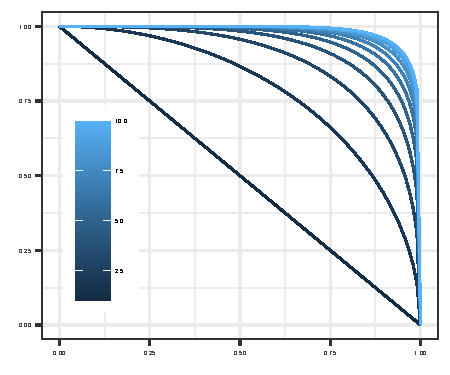
\includegraphics[width=\textwidth]{./images/p_sphere}
    \caption{${\mathbb S}_p^1$ for $p = 1,\ldots, 10$\label{fig:psphere}}
  \end{subfigure}
  %
  \begin{subfigure}[b]{0.4\textwidth}
    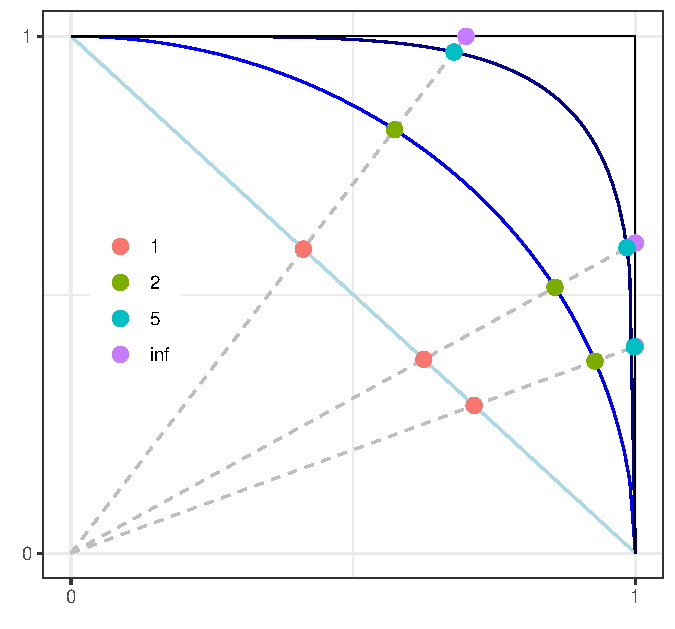
\includegraphics[width=\textwidth]{./images/p_project}
    \caption{Projection of data on ${\mathbb S}_{\infty}^1$ onto ${\mathbb S}_p^1$\label{fig:pproject}}
  \end{subfigure}
\end{figure}

A measure that is used to characterize the strength of the dependence,
  in the tail, for two random variables $Z_1$ and $Z_2$, with marginal
  distributions $F_1$ and $F_2$ is given by \citep{coles2001}
  \[
    \chi_{12} = \lim\limits_{u\uparrow 1} \prob{F_1(Z_1)>u\mid F_2(Z_2)>u}.   
  \]
  $\chi_{12}$ provides information about the distribution of extremes for the variable $Z_1$
  given that $Z_2$ is very large.  When $\chi_{12}>0$, $Z_1$ and $Z_2$ are said to
  be asymptotically dependent, otherwise they are asymptotically independent. The following result 
  provides the asymptotic dependence coefficient between two components of $\bm{Z}$ after PoT limit.
  \begin{prop}\label{ppchi}
  Suppose that $\bm{Z} = R\bm{V}$ with $R\sim Pa(1)$,
  $\prob{V_\ell > 0} = 1$ and $\expect{V_\ell}$ exists, for $\ell=1, \ldots ,d$, then
    \begin{equation}
    \label{eqn:chi_ij}
	\chi_{\jmath\ell} = \expect{\frac{V_\jmath}{\expect{V_\jmath}} \wedge \frac{V_\ell}{\expect{V_\ell}}}
    \end{equation}
  \end{prop}
  {\em Proof:}
  Denote as $F_\ell$ the marginal distribution of $Z_\ell$. To obtain $\chi_{\jmath\ell}$ we need 
  $Pr(Z_\jmath>z_\jmath,Z_\ell>z_\ell)$, where $z_\ell = F_\ell^{-1}(u) = \expect{V_\ell}/(1 - u), \;\ell=1,\dots, d$.  
  Using the fact that $V_\ell>0, \forall \ell$ almost surely, we have that the former is equal to
  \begin{equation*}
    \begin{aligned}
    &\hspace{-0.5cm}\prob{R>\frac{z_\jmath}{V_\jmath}\vee\frac{z_\ell}{V_\ell}}
    = \expect{1\wedge\left(\frac{z_\jmath}{V_\jmath}\vee\frac{z_\ell}{V_\ell}\right)^{-1}}\\
    &= \expect{\frac{V_\jmath}{z_\jmath}\wedge\frac{V_\ell}{z_\ell}}
    = (1 - u)\expect{\frac{V_\jmath}{\expect{V_\jmath}}\wedge\frac{V_\ell}{\expect{V_\ell}}},
    \end{aligned}
  \end{equation*}
  where the second identity is justified by the fact that $V_i$ is bounded and $z_i\rightarrow\infty$. The 
  proof is completed by noting that $\prob{F_i(Z_i)>u} = 1 - u. \hfill\Box$

Equation \ref{eqn:chi_ij} implies that $\chi_{\jmath\ell}>0$, and so, no asymptotic independence is possible 
  under our proposed model. For the analysis of extreme values it is of interest to calculate the multivariate 
  conditional survival function. The following result provides the relevant expression, as a function of the 
  angular measure.
  \begin{prop}
  Assume the same conditions of Proposition \ref{ppchi}.   Let $\alpha \subset \{1, \ldots ,d\}$ be a 
  collections of indexes.  Then     
  \begin{equation} \label{eqn:condsurv}
    \begin{aligned}
    &\hspace{-0.5cm}\mathrm{Pr}\left[\bigcap_{\ell \in \alpha} 
        Z_\ell > z_\ell \mid \bigcap_{\ell\not\in\alpha} Z_\ell > z_\ell\right] \\
    &= \frac{\expect{\bigwedge_{k = 1}^d 1\wedge \frac{V_k}{z_k}}}{\expect{\bigwedge_{k \not\in\alpha}1\wedge\frac{V_k}{z_k}}}.
    \end{aligned}
  \end{equation}
  \end{prop}  
  The proof uses a similar approach to the proof of Proposition \ref{ppchi}.

Equations \ref{eqn:chi_ij} and \ref{eqn:condsurv} provide relevant tools for inference on the tail 
  behavior of the joint distribution of the observations. The expressions can be readily calculated 
  within a sample-based inferential approach like the one considered in the following section.


\subsubsection{Inference for the projected Gamma mixture model}
In a sample-based inference approach, for a given iteration the Dirichlet process mixture model groups observations
    into stochastically assigned clusters, where members of a cluster share distributional parameters. Building out 
    the methods of inference for Equation~(\ref{eqn:dppg}), 
    let $n_j^{-i}$ be the number of observations in cluster $j$ not including observation $i$.  Let $J^{-i}$ be 
    the number of extant clusters, not including any singleton that observation $i$ is in. Under this model, 
    the probability of cluster membership for a given observation is proportional to
\begin{equation*}
    \text{Pr}\left[\delta_i = j\mid\ldots\right] \propto \begin{cases}
        n_j^{-i}\mathcal{PG}\left(\bm{y}_i\mid\bm{\alpha}_j,\bm{\beta}_j\right)\\ % \hspace{0.5cm} \\ % &\text{~for~}j \in \lbrace 1,\ldots,J^{-i}\rbrace\\
        \eta\int\mathcal{PG}\left(\bm{y}_i\mid\bm{\alpha}_j,\bm{\beta}_j\right)dG_0(\bm{\alpha}_j,\bm{\beta}_j),%\hspace{0.5cm} % &\text{~for~}j = J^{-i} + 1.
        \end{cases}
\end{equation*}
where the top case is iterating over extant clusters $j = 1,\ldots, J^{-i}$, and the bottom case is
    for a \emph{new} cluster. If $G_0$ is not a conjugate prior for the kernel density, the integral in the 
    above formula may not be available in closed form. We sidestep this using Algorithm 8 from \cite{neal2000}: 
    by Monte Carlo integration, we draw $m$ candidate clusters, $\bm{\alpha}_j,\bm{\beta}_j$ for
    $j = J^{-i} + 1,\ldots, J^{-i} + m$ from $G_0$. Then, we sample the cluster indicator 
    $\gamma_i$ from extant or candidate clusters, where the probability of cluster membership is proportional to
\begin{equation}
    \text{Pr}\left[\delta_i = j\mid\ldots\right] \propto \begin{cases}
        n_j^{-i}\mathcal{PG}\left(\bm{y}_i\mid\bm{\alpha}_j,\bm{\beta}_j\right)\\ % \hspace{0.5cm}  % &\text{~for~}j \in \lbrace 1,\ldots,J^{-i}\rbrace\\
        \frac{\eta}{m}\mathcal{PG}\left(\bm{y}_i\mid\bm{\alpha}_j,\bm{\beta}_j\right). % \hspace{0.5cm} &\text{~for~}j \in \lbrace J^{-i} + 1,\ldots, J^{-i} + m\rbrace.
        \end{cases}
\end{equation}
Again, the top case is iterating over extant clusters, and now the bottom case is iterating 
    over new \emph{candidate} clusters.  If a candidate cluster is selected,
%{\bf you first have to say that you sample from this distribution. What is the ``candidate cluster''?}
    then $\gamma_i = J = J^{- i} + 1$, and the associated cluster parameters are saved.

A key feature of the the projected Gamma distribution is its computational properties. We augment 
$\mathcal{PG}(\bm{y}_i\mid\bm{\alpha}_i,\bm{\beta}_i) $ by introducing a latent radial component $r_i$, 
for each observation. Using Equation \eqref{joint} we observe that the 
full conditional of $r_i$ is easy to sample from, as it is given as
\begin{equation}
    r_i\mid\bm{\alpha}_i,\bm{\beta}_i \sim \mathcal{G}\left(r_i \bigmid \sum_{\ell = 1}^d\alpha_{i\ell}, \sum_{\ell = 1}^d\beta_{\ell} y_{i\ell}\right).
\end{equation}
Moreover,  the full conditional for $\bm{\alpha}_j,\bm{\beta}_j$ is then proportional to
\begin{equation}
    \begin{aligned}
    &\hspace{-1cm}f(\bm{\alpha}_j,\bm{\beta}_j\mid \bm{Y},\bm{r},\bm{\delta},\ldots) \\
    &\propto \prod_{i:\gamma_i = j}\prod_{\ell = 1}^d\mathcal{G}\left(r_iy_{i\ell}\mid\alpha_{j\ell},\beta_{j\ell}\right) \\
    &\hspace{0.5cm} \times dG_0(\bm{\alpha}_j,\bm{\beta}_j).
    \end{aligned}
\end{equation}
Note that the ordering of the products can be reversed in the likelihood, indicating that given $\bm{r}$, 
the likelihood becomes separable by dimension.
We first consider a centering distribution given by a product of independent Gammas:
\begin{equation}
    \begin{aligned}
    &\hspace{-0.3cm}G_0(\bm{\alpha}_j,\bm{\beta}_j\mid \bm{\xi},\bm{\tau},\bm{\zeta},\bm{\sigma}) \\
    &= \prod_{\ell = 1}^d\mathcal{G}(\alpha_{j\ell}\mid \xi_{\ell},\tau_{\ell})\times\prod_{\ell = 2}^d\mathcal{G}(\beta_{j\ell}\mid\zeta_{\ell},\sigma_{\ell}).
    \end{aligned}
\end{equation}
This model is completed with independent Gamma priors on $\xi_{\ell}$, $\tau_{\ell}$, $\zeta_{\ell}$, $\sigma_{\ell}$.  We also assume a Gamma prior on $\eta$, that is updated via the procedure outlined in \cite{escobar1995}.  We refer to this model as the \emph{projected Gamma--Gamma} (PG--G) model.  An advantage of the PG--G model is that, thanks to conjugacy, the rate parameters can easily be integrated out for inference on $\bm{\alpha}_j$.  Then, the full conditional for $\alpha_{j\ell}$ takes the form
\begin{equation}
    \label{eqn:alphalupdate}
    \begin{aligned}
    &\hspace{-0.5cm}\pi(\alpha_{j\ell}\mid \bm{r},\bm{Y},\bm{\gamma},\xi_\ell,\tau_\ell,\zeta_\ell,\sigma_\ell) \\
    &\propto \frac{\left(\prod_{i:\gamma_i = j}r_iy_{i\ell}\right)^{\alpha_{j\ell} - 1}\alpha_{j\ell}^{\xi_\ell - 1}e^{-\tau_\ell \alpha_{j\ell}}\times}{\Gamma^{n_j}(\alpha_{j\ell})} \\
    &\hspace{0.5cm}\times \frac{\Gamma\left(n_j\alpha_{j\ell} + \zeta_{\ell}\right)}{\left(\sum_{i:\gamma_i = j}r_iy_{i\ell} + \sigma_{\ell}\right)^{n_j\alpha_{j\ell} + \zeta_{\ell}}}
    \end{aligned}
\end{equation}
for $\ell = 2,\ldots,d$.  For $\ell = 1$, as $\beta_{1} := 1$, the full conditional takes the simpler form
\begin{equation}
    \label{eqn:alpha1update}
    \begin{aligned}
    &\hspace{-0.5cm}\pi(\alpha_{j1}\mid\bm{r},\bm{Y},\bm{\gamma},\xi_1,\tau_1) \\
    &\propto \frac{\left(\prod_{i:\gamma_i = j}r_iy_{i1}\right)^{\alpha_{j1} - 1}\alpha_{j1}^{\xi_1 - 1}e^{-\tau_1\alpha_{j1}}}{\Gamma^{n_j}(\alpha_{j1})}.
    \end{aligned}
\end{equation}
Samples of $\alpha_{j\ell}$ can thus be obtained using a Metropolis step. In our analysis, we first transform $\alpha_{j\ell}$ to the log scale, and use a normal proposal density.
The full conditional for $\beta$ is 
\begin{equation}
    \label{eqn:betafc}
    \begin{aligned}
    &\hspace{-0.5cm}\beta_{j\ell}\mid\bm{r},\bm{Y},\alpha,\zeta_{\ell},\sigma_{\ell} \\
    &\sim \mathcal{G}\left(\beta_{j\ell}\bigmid n_j\alpha_{j\ell} + \zeta_\ell, \sum_{i:\gamma_i = j}r_iy_{i\ell} + \sigma_{\ell}\right),
    \end{aligned}
\end{equation}
for $\ell = 2,\ldots, d$.  Updating $\beta_{j\ell}$ is done via a Gibbs step.  The hyper-parameters $\xi_{\ell},\tau_{\ell},\zeta_{\ell},\sigma_{\ell}$ follow similar Gamma-Gamma update relationships.  We also explore a restricted form of this model, where $\beta_{\ell} = 1$ for all $\ell$.  Under this model, we use the full conditional in Equation~(\ref{eqn:alpha1update}) for all $\ell$, and omit inference on $\bm{\zeta},\bm{\sigma}$.  We refer to this model as the \emph{projected restricted Gamma--Gamma} (PRG--G) model.

The second form of centering distribution we explore is a multivariate log-normal distribution on the shape parameters $\bm{\alpha}_j$, with independent Gamma $\beta_{j\ell}$ rate parameters.  
\begin{equation}
    \begin{aligned}
    &\hspace{-0.5cm}G_0\left(\bm{\alpha}_j,\bm{\beta}_j\mid\bm{\mu},\bm{\Sigma},\zeta,\sigma\right) \\
    &=\mathcal{LN}\left(\bm{\alpha}_j\mid\bm{\mu},\bm{\Sigma}\right)\times\prod_{\ell = 2}^d\mathcal{G}\left(\beta_{j\ell}\mid\zeta_{\ell},\sigma_{\ell}\right).
    \end{aligned}
\end{equation}
This model is completed with a normal prior on $\bm{\mu}$, an inverse Wishart prior on $\bm{\Sigma}$, and Gamma priors on $\zeta_{\ell}$ and $\sigma_{\ell}$, and $\eta$.  This model is denoted as the \emph{projected Gamma--log-normal} (PG--LN) model.  We also explore a restricted Gamma form of this model as above, where $\beta_{\ell} = 1$ for all $\ell$.  This is denoted as the \emph{projected restricted Gamma--log-normal} (PRG--LN) model.  Updates for $\bm{\alpha}$ can be accomplished using a joint Metropolis step, where $\beta_{j\ell}$ for $\ell = 2,\ldots,d$ have been integrated out of the log-density.  That is,
\begin{equation*}
    \begin{aligned}
    &\hspace{-0.5cm}\pi(\bm{\alpha}_j\mid\bm{Y},\bm{r},\bm{\delta},\bm{\mu},\bm{\Sigma},\bm{\zeta},\bm{\sigma})\\
    &\propto \exp\left\lbrace-\frac{1}{2}(\log\bm{\alpha}_j - \mu)^T\bm{\Sigma}^{-1}(\log\bm{\alpha}_j - \mu)\right\rbrace \\
    &\hspace{0.5cm}\times\frac{1}{\prod_{\ell = 1}^d\alpha_{j\ell}}\times \frac{\left(\prod_{i:\gamma_i = j}r_iy_{i1}\right)^{\alpha_{j1} - 1}}{\prod_{\ell = 1}^d\Gamma^{n_j}(\alpha_{j\ell})}\\
    &\hspace{0.5cm}\times \prod_{\ell = 2}^d\frac{\Gamma\left(n_j\alpha_{j\ell} + \zeta_{\ell}\right)}{\left(\sum_{i:\gamma_i = j}r_iy_{i\ell} + \sigma_{\ell}\right)^{n_j\alpha_{j\ell} + \zeta_{\ell}}}
    \end{aligned}
\end{equation*}
The inferential forms for $\beta_{j\ell}$ and its priors are the same as for PG--G.  The 
  normal prior for $\mu$ is conjugate for the log-normal $\bm{\alpha}_j$, and can be sampled
  via a Gibbs step.  Finally, the inverse Wishart prior for $\Sigma$ is again conjugate to
  the log-normal $\bm{\alpha}_j$, implying that it can also be sampled via a Gibbs step.

% EOF


% EOF

\section{Scoring criteria for distributions in ${\mathbb S}_\infty^{d-1}$\label{sec:evaluation}}

In order to assess and compare the estimation of a distribution on ${\mathbb S}_\infty^{d-1}$ we consider the theory of proper scoring rules developed in \cite{gneiting2007}.
As mentioned in Section~\ref{subsec:projgamma}, our approach does not provide a density on ${\mathbb S}_{\infty}^{d-1}$, restricting our ability to construct model selection criteria to sample-based approaches.  We consider two scoring methods:  \emph{posterior predictive loss} (PPL) introduced in \cite{gelfand1998}, and \emph{energy score} (ES) introduced in \cite{gneiting2007}.

\subsection{Posterior predictive loss}
The posterior predictive loss criterion is introduced in \cite{gelfand1998}.  When we
  assume a squared error loss function, then for the $i$th observation, the posterior predictive
  loss criterion is computed as
  \begin{equation}
    \label{eq:ppl}
      S_{\text{PPL}}^k\left(P,x_i\right) = \text{Var}_P\left(X_i\right) + \frac{k}{k+1}\left(\text{E}_P\left[X_{i}\right] - x_i\right)^2
  \end{equation}
  where $X_i$ is a random variable from the posterior predictive distribution for $x_i$.  The
  scalar $k$ is a weighting factor that scales the importance of goodness of fit
  relative to precision.  In fact a small $\text{Var}(X_{i})$ indicates high
  precision, and a small $(\text{E}[X_{i}] - x_{i})^2$  indicates a good fit.  In our analysis,
  we take the limit as $k\to\infty$, weighting both
  equally. Overall, the smaller the score, the better.  Note that the PPLC score is defined 
  for a univariate distribution.  As we are dealing
  with a multivariate distribution, we will be taking the posterior predictive loss
  summed over all dimensions.  That is,
  \begin{equation}
    \label{eq:ppl2}
      S_{\text{PPL}}\left(P,\bm{x}_i\right) = \frac{1}{d}\sum_{\ell = 1}^d\left[\text{Var}_P\left(X_{i\ell}\right) + \left(\text{E}_P\left[X_{i\ell}\right] - x_{i\ell}\right)^2\right] .
  \end{equation}
  We report the average $S_{\text{PPL}}$ taken from all observed data.

\subsection{Energy score}
We focus on \emph{energy scores} defined for a general probability distribution $P$, with finite expectation, as 
    \begin{equation}
    \label{eq:es}
    \text{S}_{\text{ES}}\left(P, \bm{x}_i\right) =  \text{E}_p g\left(\bm{X}_i, \bm{x}_i\right) -
                                    \frac{1}{2}\text{E}_p g\left(\bm{X}_i,\bm{X}_i^{\prime}\right),
    \end{equation}
where $g$ is a kernel function. The score defined in Equation \eqref{eq:es} can be evaluated
  using samples from $P$, with the help of the law of large numbers.
  Moreover, Theorem~4 in \cite{gneiting2007}, states that if $g(\cdot,\cdot)$ is a negative 
  definite kernel, then $\text{S}(P,\bm{x})$ is a \emph{proper} scoring rule.  Recall that a 
  real valued function $g$ is a negative definite kernel if it is symmetric in its arguments, 
  and $\sum_{i=1}^n\sum_{j=1}^na_ia_jg(x_i,x_j)\leq 0$ for all positive integers $n$, and any 
  collection $a_1,\ldots,a_n\in{\mathbb R}$ such that  $\sum_{i = 1}^na_i = 0$.  

In a Euclidean space, these conditions are satisfied by the Euclidean distance. However, in
  ${\mathbb S}_{\infty}^{d-1}$, Euclidean distance will tend to under-estimate the actual 
  distance required to travel between two points.  Let
\begin{equation*}
    {\mathbb C}_{\ell}^{d-1} = \lbrace \bm{x} : \bm{x} \in {\mathbb S}_{\infty}^{d-1}, x_{\ell} = 1\rbrace
\end{equation*}
comprise the $\ell$th \emph{face}.  For points on the same face, Euclidean distance 
  corresponds to the length of the shortest possible path in ${\mathbb S}_{\infty}^{d-1}$.  
  For points on different faces, the Euclidean distance is a lower bound for that length.

For a finite $p$, the shortest connecting path between two points in ${\mathbb S}_p^{d-1}$
  is the minimum geodesic; its length satisfying the definition of a distance.  Thus its
  length can be used as a negative definite kernel for the purpose of defining an energy
  score. Unfortunately as $p\to\infty$ the resulting surface ${\mathbb S}_{\infty}^{d-1}$
  is not differentiable, implying that routines to calculate geodesics are not readily
  available.  However, as ${\mathbb S}_{\infty}^{d-1}$ is a portion of of a $d$-cube, we
  can borrow a result from geometry \citep{pappas1989} stating that the length of the
  shortest path between two points on a geometric figure corresponds to the length of a
  straight line drawn between the points on an appropriate unfolding, rotation, or \emph{net} of the figure from a $d$-dimensional to a $d-1$-dimensional space.  The optimal net will have the shortest straight line between the points, as long as that line is fully contained within such net. As ${\mathbb S}_{\infty}^{d-1}$ has $d$ faces---each face pairwise adjacent, there are $d!$ possible nets.  However, we are only interested in nets that begin and end on the source and destination faces respectively.  That reduces the number of nets under consideration to $\sum_{k = 0}^{d-2}\binom{d-2}{k}$.  This is still computationally burdensome for a large number of dimensions.  

To reduce the computations needed to calculate the energy score we define a kernel as {\bf Please write a clearer description here.} our kernel an upper bound on distance between points on separate faces as the length of the path from the source point, to an optimal point on the intersection between faces, to the destination point.
\begin{prop}\label{prop:g}
Let $\bm{a} \in {\mathbb C}_{\ell}^{d-1}$, and $\bm{b} \in {\mathbb C}_{\jmath}^{d-1}$, for $\ell, \jmath \in \{1, \ldots , d\}$. Define $g$ as
\[  
    g(\bm{a},\bm{b}) = \min_{\bm{c} \in{\mathbb C}_{\jmath}^{d-1}\cap{\mathbb C}_{\ell}^{d-1}}\left\{ 
        \pnorm{\bm{c}-\bm{a}}{2} + \pnorm{\bm{b}-\bm{c}}{2} \right\}.
\]
Then $g$  is negative definite kernel.
\end{prop}

{\em Proof:}
When $\bm{a}$ and $\bm{b}$ are on the same face, then $\ell = \jmath$, and $g$ is the Euclidean distance between $\bm{a}$ and $\bm{b}$, which is a  negative definite kernel.  When $\bm{a}$ and $\bm{b}$ are on separate
  faces, let 
  \[\bm{d} = 
    \argmin_{\bm{c} \in{\mathbb C}_{\jmath}^{d-1}\cap{\mathbb C}_{\ell}^{d-1}}\left\{ 
        \pnorm{\bm{c}-\bm{a}}{2} + \pnorm{\bm{b}-\bm{c}}{2} \right\}.
  \]
  We have that $g(\bm{a}, \bm{b}) = g(\bm{b}, \bm{a})$ due to the uniqueness of $\bm{d}$ and the symmetry of the Euclidean distance. Additionally, given $n$ and  a collection $\alpha_1,\ldots,\alpha_n\in{\mathbb R}$ such that  $\sum_{i = 1}^n\alpha_i = 0$, then, 
  \begin{equation*}
    \begin{aligned}
      \sum_{i = 1}^n\sum_{j = 1}^n \alpha_i\alpha_j g(\bm{x}_1,\bm{x}_2) &= \sum_{i = 1}^n\sum_{j = 1}^n \alpha_i\alpha_j \bigg[\pnorm{\bm{d} - \bm{x}_1}{2} + \pnorm{\bm{x}_2 - \bm{d}}{2}\bigg]\\
      &= \sum_{i = 1}^n\sum_{j = 1}^n \alpha_i\alpha_j\pnorm{\bm{d} - \bm{x}_1}{2} + \sum_{i = 1}^n\sum_{j = 1}^n \alpha_i\alpha_j\pnorm{\bm{x}_2 - \bm{d}}{2} \leq0,
    \end{aligned}
  \end{equation*}
  as the Euclidean norm is a negative definite kernel.$\hfill\Box$
 
Evaluating $g$ as defined in Proposition \ref{prop:g} requires the solution of a $(d-2)$-dimensional 
  optimization problem.  The following proposition provides a straightforward solution.
\begin{prop}
    Let $\bm{a} \in {\mathbb C}_{\ell}^{d-1}$, and $\bm{b} \in {\mathbb C}_{\jmath}^{d-1}$, for $\ell, \jmath \in \{1, \ldots , d\}$.  For $\ell\neq \jmath$, the 
  transformation $P_{\jmath\ell}(\cdot)$ required to rotate the $\jmath$th face along the $\ell$th axis 
  produces the vector $\bm{b}^\prime$, where
  \begin{equation}
    \label{eqn:rotation}
     \bm{b}^{\prime}_i = P_{\jmath\ell}(\bm{b}) = 
    \begin{cases}
        b_{i} &\text{for }i\neq \jmath,\ell\\
        1 &\text{for }i = \ell\\
        2 - b_{\ell} &\text{for }i = \jmath
    \end{cases}.
  \end{equation}
  Then $g(\bm{a},\bm{b}) = \pnorm{\bm{a} - \bm{b}^{\prime}}{2}$.
\end{prop}
{\em Proof:}
Notice that for 
  $\bm{c} \in {\mathbb C}_{\jmath}^{d-1}\cap{\mathbb C}_{\ell}^{d-1}$,
     $\pnorm{\bm{b} - \bm{c}}{2} =  \pnorm{\bm{b}^{\prime} - \bm{c}}{2}$. {\bf This is true just because you do the math, the invariance of Euclidean norms is not needed.} Then, recalling the definition of $\bm{d}$ in the proof of Proposition \ref{prop:g}, we have that
  \begin{equation*}
    \begin{aligned}
    g(\bm{a}, \bm{b}) &= \pnorm{\bm{a} - \bm{d}}{2} + \pnorm{\bm{b} - \bm{d}}{2}\\
    &= \pnorm{\bm{a} - \bm{d}}{2} + \pnorm{\bm{b}^{\prime} - \bm{d}}{2} = \pnorm{\bm{a} - \bm{b}^{\prime}}{2}.
    \end{aligned}
  \end{equation*}
  The last equality is due to the fact that $\bm{a}$ and $\bm{b}'$ belong to the same hyperplane.
  $\hfill\Box$

We report the average $S_{\text{ES}}$ taken across all observed data.  In this form, the interpretation of $S_{\text{ES}}$ is similar to that of $S_{\text{PPL}}$: the smaller the score, the better.
% EOF



\section{Data illustrations\label{sec:results}}

\subsection{Simulations\label{subsec:simulated}}
To evaluate our proposed approach for angular measure estimation 
we consider simulated datasets on $\mathcal{S}_{\infty}^{d-1}$, for 
$d$ ranging between 3 and 20. We generated each dataset from a mixture of projected Gammas, with the number of mixture components
  ranging between 3 and 12.  The generation procedure is detailed in Algorithm~\ref{algo:simulated}.
  \begin{algorithm}[ht]
    \caption{Simulated Angular Dataset Generation Routine\label{algo:simulated}}
    \For{$n_{\text{mix}}$ in $[3, 6, 9, 12]$}{
      Generate $n_{\text{mix}} \times 20$ shape Parameters $\alpha$\\
      Generate $n_{\text{mix}} \times 20$ Rate Parameters $\beta$\\
      Generate $500$ Mixture Component Identifiers $\delta$\\
      \For{$i$ in $1,\ldots,500$}{
        Generate ${\bf X}_i \sim \prod_{\ell = 1}^d\text{Ga}\left(X_{il}\mid\alpha_{\delta_i,l},\beta_{\delta_i, l}\right)$
        }
      \For{$n_{\text{col}}$ in $[3,6,12,20]$}{
        Project columns 1 to $n_{\text{col}}$ of ${\bf X}$ onto 
        $\mathcal{S}_{\infty}^{n_{\text{col}} - 1}$ and save.
        }
    }
  \end{algorithm}
Each one of the shape parameters $\alpha$ were generated 
$\alpha = \alpha_0 + \alpha_1$ where
  $\alpha_0 \sim \text{Unif}(\alpha_0\mid 0,4)$, $\alpha_1\sim \text{Gamma}(\alpha_1\mid 1,1)$.
The scale parameters $\beta$ were obtained as $\beta\sim\text{Unif}(\beta\mid 0.25, 2.5)$.

% \begin{figure}[ht]
%   \caption{Simulation Energy Score versus Column Count, by Mixture Component Count. Lower is better.\label{fig:simes}}
%   \centering
%   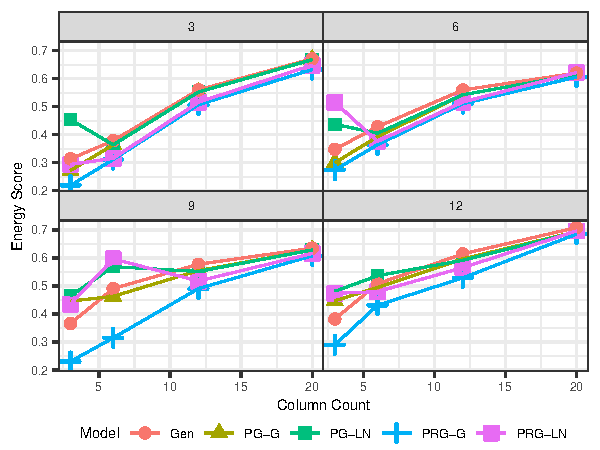
\includegraphics[width=0.8\textwidth]{./images/simulation_es}
% \end{figure}

\begin{figure}[ht]
\begin{center}
  \begin{subfigure}[b]{0.48\textwidth}
    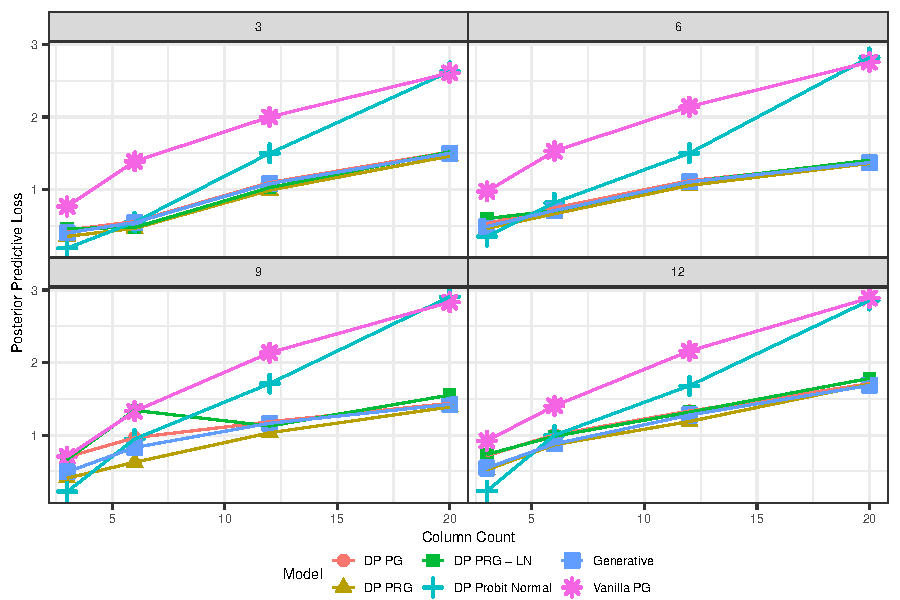
\includegraphics[width=\textwidth]{./images/simulation_ppl}
    \caption{Posterior Predictive Loss\label{fig:simppl}}
  \end{subfigure}
  %
  \begin{subfigure}[b]{0.48\textwidth}
    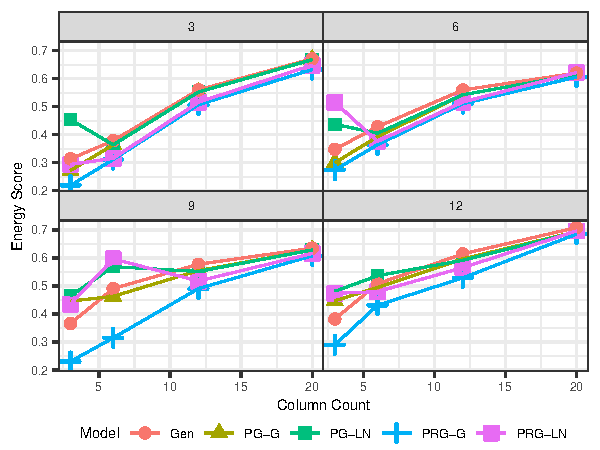
\includegraphics[width=\textwidth]{./images/simulation_es}
    \caption{Energy Score\label{fig:simes}}
  \end{subfigure}
  \caption{Scores for the simulated datasets calculated using different models:
  GEN - baseline; PG - mixture of projected gammas; PRG - mixture of projected restricted gamma; PRG--LN - mixture of projected restricted gammas with log-normal prior.}
\end{center}
\end{figure}

Figure~\ref{fig:simes}, shows two sets of panels that illustrate the comparison
between four different models used to fit the simulated data. We produced 16 
different data sets, one for each of four different numbers of mixture components 
and four different dimensions. We considered three different models: DP mixtures 
of projected gamma; Projected restricted gamma; and projected restricted gamma 
with a multivariate log-normal prior. We calculated $S^\infty_{\text{PPL}}$ and 
$S_{\text{ES}}$ using predictive samples from each of fitted models. To provide 
a comparative baseline, we calculated the scores using samples from generated 
directly using the same model and parameters that produced the simulated 
observations. The results are denoted as \emph{Gen} in the figure. 
We observe that the projected
  restricted Gamma model dominates in most situations, but the difference between projected restricted
  Gamma and the other gamma-based models tends to shrink as the number of dimensions increases.
  Alternatively, that difference appears to grow as the number of mixture components increases. The results from both scoring criteria are pretty comparable.

% \begin{figure}[ht]
%   \caption{Simulation posterior predictive loss versus column count, by mixture component count.\label{fig:simppl}}
%   \centering
%   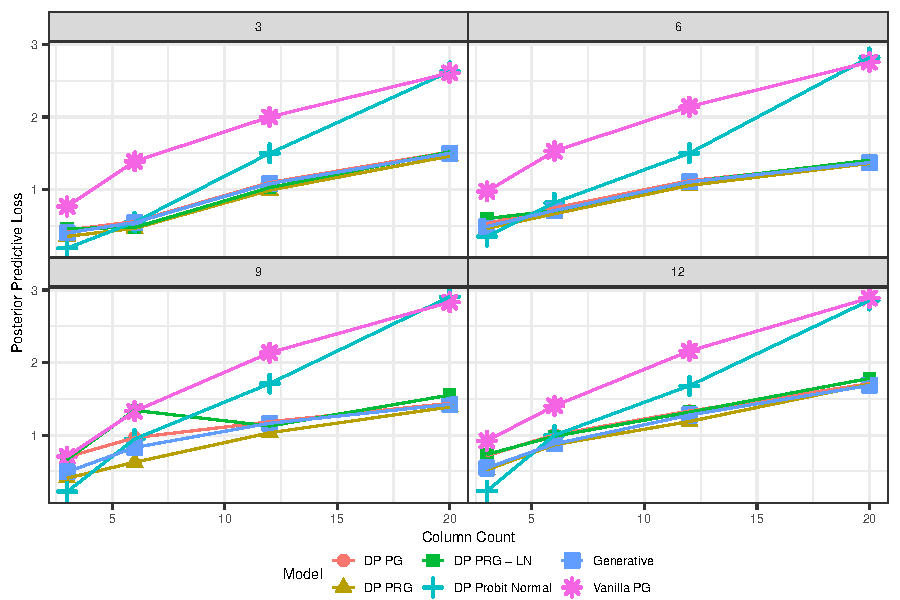
\includegraphics[width=0.8\textwidth]{./images/simulation_ppl}
% \end{figure}

We frequently see all of the gamma-based mixture models accomplish a lower energy score than the generative
  distribution.  As \cite{nunez2019} noted, the projected Gamma model is very flexible and can generate
  multimodal distributions from a single mixture component.  When we allow a mixture model, we allow
  the possibility to break those modes into two different mixture components.  This will tend to
  result in a better energy score, as posterior predictive replicates for a given observation in a local
  model will tend to be concentrate in that local mode rather than being spread between multiple
  modes.  As for the dominance of projected restricted Gamma, By specifying $\beta_{\ell} := 1$ for all
  $l$, if there were multi-modal mixture components, we are in effect breaking the mixture components
  into separate modes. As for whether this represents \emph{overfitting}, If we had reason to
  believe that the generative distribution for real data followed this form, then such a case could
  be made.  However, we are using projected Gamma as a parametric stand-in for an unknown distribution.
  In this sense, the argument for overfitting is less clear.
  {\bf This paragraph is not very clear. Please make an effort to tell the story more clearly.}

\subsection{Integrated Vapor Transport\label{subsec:ivt}}
The \emph{integrated vapor transport} (IVT) is a two component vector 
that tracks the flow of the total water volume in a column of air 
over a given area \citep{ralph2017}.  IVT is increasingly used in the study of atmospheric rivers because of its direct 
relationship with orographically induced precipitation
\citep{neiman2009water}. Atmospheric rivers (AR) are elongated areas of high 
local concentration of water vapor in the atmosphere that transport water
from the tropics around the world. AR can cause extreme 
precipitation,  something that usually associated with very large values
of the IVT magnitude over a whole geographical area. In spite of this, AR
are fundamental for the water supply of areas like California. Thus the
importance of understanding the extreme behavior of IVT, including 
extreme tail dependence. We consider datasets that correspond to IVT
estimated at two different spatial resolutions. The coarse resolution dataset
is obtained from the European Centre for Medium-Range Weather Forecasts
(ECMWF) Interim reanalysis (ERA-Interim) \citep{berrisford2011atmospheric,dee2011era}. 
The high resolution dataset corresponds to the latest ECMWF 
observational product, ERA5  \citep{hersbach2020era5}. 

Our data corresponds to daily average values for the IVT magnitude
along the coast of California.  The ERA-Interim data used covers the time period 
1979 through 2014 (37 years) omitting leap days, and provides 8 grid cells.  The ERA5 data
covers the time period 1979 through 2019 (42 years) with the same restriction, and provides 
47 grid cells.  This gives us the opportunity to illustrate the performance of our method 
in multivariate settings of very different dimensions. Figure~\ref{fig:gridlocs} provides a visual representation of the area these grid cells represent.

\begin{figure}[ht]
    \begin{center}
    \begin{subfigure}[b]{0.48\textwidth}
        \centering 
        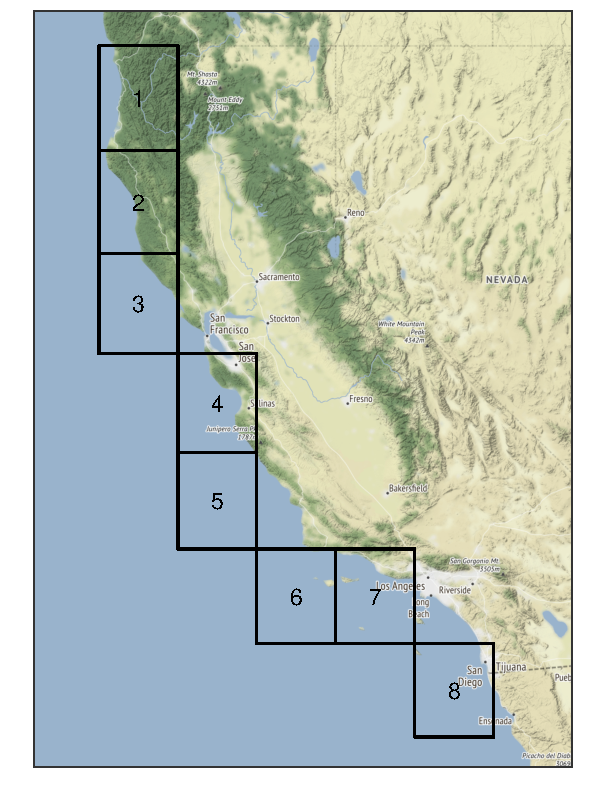
\includegraphics[height=3in]{./images/erai_grid}
    \end{subfigure}
    %
    \begin{subfigure}[b]{0.48\textwidth}
        \centering
        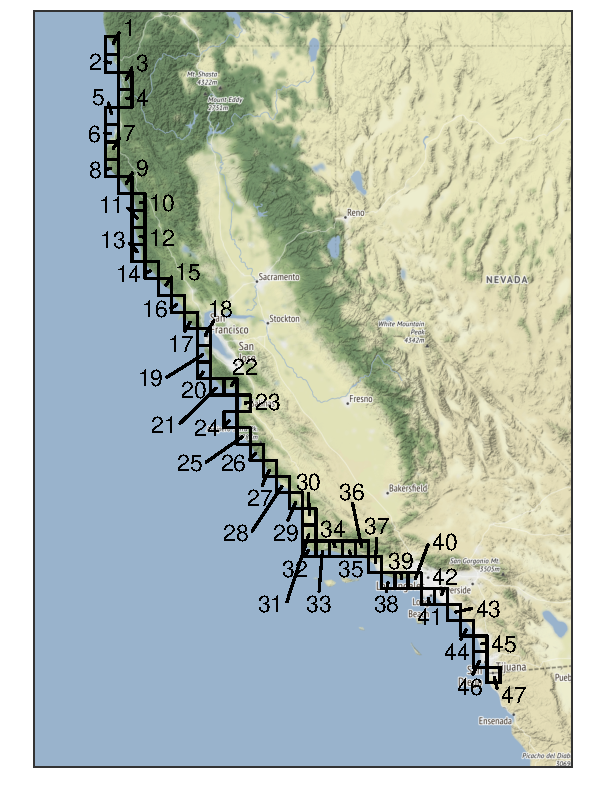
\includegraphics[height=3in]{./images/era5_grid}
    \end{subfigure}
    \caption{Grid cell locations for ERA-Interim (left) and ERA5 (right).\label{fig:gridlocs}}
    \end{center}
\end{figure}

\begin{algorithm}[h]
  \KwResult{$\bm{ r},\bm{v} : r_i \sim \text{Pareto}(1)$, $\bm{ v}_i \in {\mathbb S}_{\infty}^{d-1}$}
  \For{$\ell = 1,\ldots,d$}{
    Set $b_{t,\ell} = \hat{F}_{\ell}^{-1}\left(1 - \frac{1}{t}\right)$.\\
    With $\bm{ x}_{\ell} > b_{t,\ell}$, fit $a_{\ell}$, $\chi_{\ell}$ via MLE according to generalized Pareto likelihood.\\
    }
  \For{$i = 1,\ldots,n$}{
    Define $z_{i,\ell} = \left(1 + \xi_{\ell}\frac{x_{i,\ell} - b_{t,\ell}}{a_{\ell}}\right)_{+}^{1/\xi_{\ell}}$\\
    Define $r_i = \pnorm{\bm{ z}_i}{\infty}$, $\bm{ v}_i = \frac{\bm{ z}_i}{\pnorm{\bm{ z}_i}{\infty}}$\\
    }
  Subset $\bm{ r},\bm{ v}$ such that $r_i \geq 1$\\
  \If{declustering}{
    \For{$i = 1,\ldots,n$}{
      If $r_i \geq 1$ and $r_{i-1} \geq 1$, drop the lesser (and associated $v_i$) from data set.\\
    }
  }
 \caption{Data preprocessing to isolate and transform data exhibiting extreme behavior.  $r_i$
   represents the radial component, and $\bm{v}_i$ the angular component.  The declustering
   portion is relevant for data correlated in time.\label{algo:processing}}
\end{algorithm}

Fitting our models to the IVT data requires some pre-processing. First, we subset the data to the rainy
  season, which in California runs roughly from November to March.  Following the approach described in Section \ref{sec:methodology} we estimate the shape and scale parameters of a univariate GP, in each dimension, using maximum likelihood. We set the threshold in each dimensions $\ell$ as  $b_{t,\ell} = \hat{F}_{\ell}^{-1}(1 - t^{-1})$, where $\hat{F}$ is the empirical CDF and $t=20$, that corresponds to the $95$ percentile. We then use the transformation in Equation \eqref{eqn:standardization} to standardize the observations.
  Dividing each standardized observation by its $\mathcal{L}_{\infty}$ 
  norm, we obtain a projection onto $\mathcal{S}_{\infty}^{d-1}$. As the data correspond to a daily time series, the observations are temporally correlated.  For each group of consecutive standardized vectors $z_i$ such  that  $\inorm{z_i} > 1$, we retain only the vector 
  with the largest $\mathcal{L}_{\infty}$ norm.  The complete procedure is outlined in
  Algorithm~\ref{algo:processing}.  After subsetting the ERA-Interim data to the rainy season we 
  have $5587$ observations. This reduces to $511$ observations after processing and declustering.  
  For the ERA5 data, after subsetting we have $6342$ observations, which reduces to $532$ observations after 
  processing and declustering.  We fit the PG--G, PRG--G, PG--LN, and PRG--LN models to both datasets.
  {\bf At this point it would be nice to include a figure with a plot of the data after all the pre-processing. You show a couple of panels for the ERA-Iterim and a couple of the ERA5.}
  \makenote{Do you mean marginal histograms, or, like, a couple selected ternary scatter-plots?}

\begin{table}[t]
  \centering
  \caption{Model comparison metrics: Posterior~Predictive~Loss~($S_{\text{PPL}}$) and 
    Energy~Score~($S_{\text{ES}}$) criteria from fitted models against the IVT data.  
    Lower is better. \label{tab:dev}}
  
\begin{tabular}{ccccc}
\toprule
\multicolumn{1}{c}{ } & \multicolumn{2}{c}{dim = 8} & \multicolumn{2}{c}{dim = 47} \\
\cmidrule(l{3pt}r{3pt}){2-3} \cmidrule(l{3pt}r{3pt}){4-5}
Model & PPL & ES & PPL & ES\\
\midrule
PRG & 0.195 & 0.170 & 1.623 & 0.675\\
PRG-LN & 0.232 & 0.192 & 1.400 & 0.582\\
PG & 0.787 & 0.418 & 5.040 & 1.374\\
\bottomrule
\end{tabular}
\end{table}

Table~\ref{tab:dev} shows the values of the estimated posterior predictive loss and energy scores for the different models considered. We observe that, as in the case of the simulation study shown in Figures~\ref{fig:simes}, the preferred model is the projected restricted 
  gamma models.  Penalization for the unrestricted gamma model is 
  stronger for the real data than for the simulated data. We also observe that
  the restricted gamma model with the log-normal prior performs significantly better 
  than the restricted gamma model with the gamma prior on the higher dimensional data. This is the opposite of the result obtained in the simulation example.

\begin{figure}[ht]
    \centering
    \caption{Pairwise extremal dependence coefficients for IVT data using the PRG--G model.\label{fig:chi_ij}}
    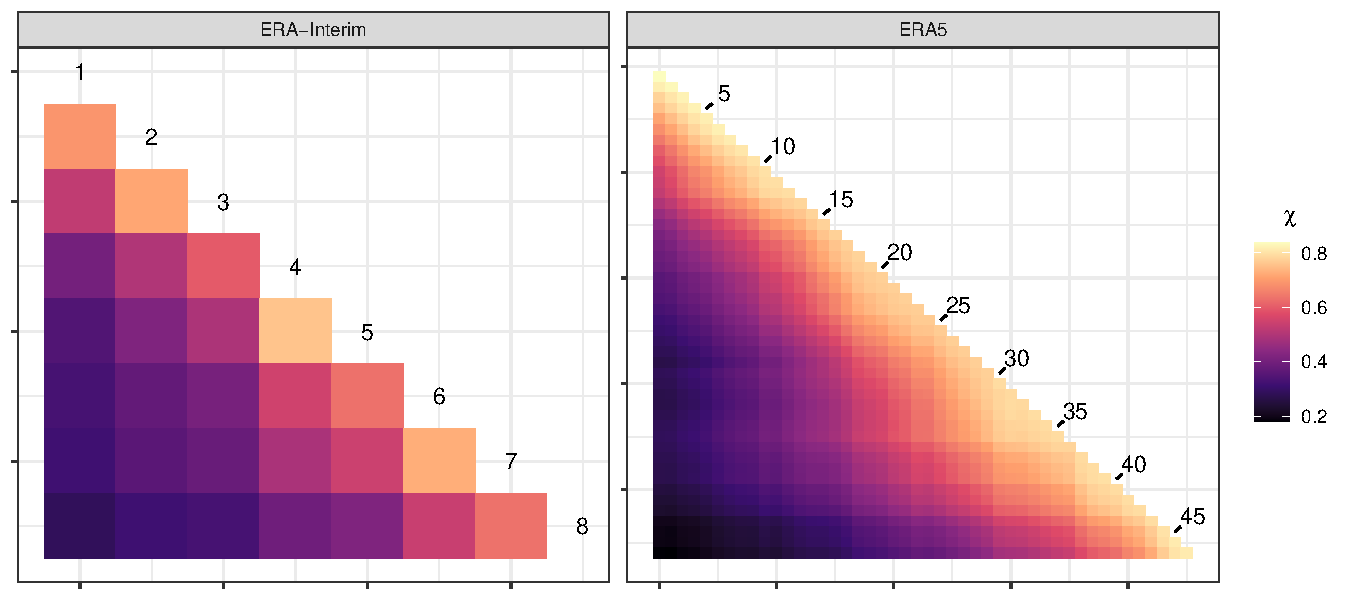
\includegraphics[width=0.9\textwidth]{./images/chi_ij_c}
\end{figure}

We consider an exploration of the pairwise extremal dependence using Monte Carlo estimates of the 
  coefficients in  Equation~\ref{eqn:chi_ij}. For this we use samples obtained fromn the PRG--G model.
  Figure~\ref{fig:chi_ij} provides a graphical analysis of the results. 
  The coefficients achieve values between $0.286$ and $0.759$ for the ERA-Interim data and 
  between $0.181$ and $0.840$ for the ERA5 data.  The greater range in dependence scores observed 
  with the ERA5 data speaks to the greater granularity of the ERA5 data. Distance between locations 
  mostly determines the strength of the pairwise asymptotic dependence. The highest coefficients 
  are $0.759$ for locations 4 and 5 in the ERA-Interim data and
  $0.840$ for locations 1 and 2 in the ERA5 data.  Clearly, pairwise asymptotic
  dependence coefficients tell a limited story, as a particular dependence may include
  more than two locations.   We can, however, glean some information from the patterns that emerge in
  two dimensions.  For the ERA-Interim data, we observe a possible cluster between cells 5-8, indicating a
  strong dependence among these cells.  Analogously, for the ERA5 data, we observe three possible groups  of locations.

\begin{figure}[ht]
    \centering
    \caption{Conditional survival curves for selected locations, conditioning on all other dimensions at greater than 90th percentile (fitted)\label{fig:condsurv1d}. The left panel uses original units. Right panel uses standardized units.}
    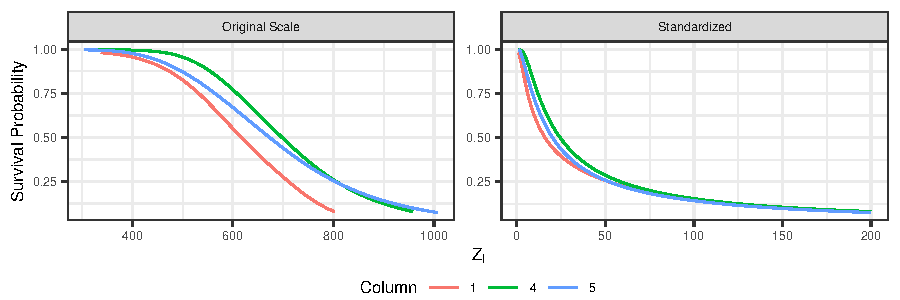
\includegraphics{./images/condsurv_1d}
\end{figure}

\begin{figure}[htb]
    \centering
    \caption{Pairwise conditional survival curves for selected locations, conditioning on all other dimensions at greater than 90th percentile (fitted)\label{fig:condsurv2d}}
    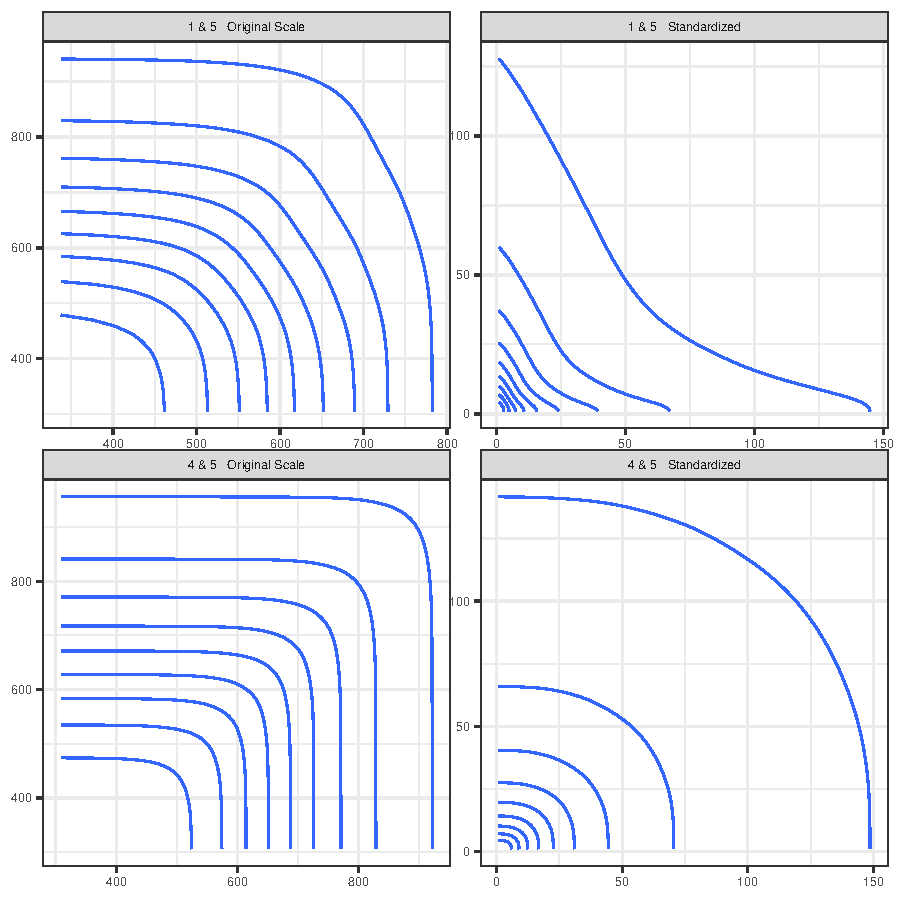
\includegraphics[height=5in, width=5in]{./images/condsurv_2d}
\end{figure}

Figure~\ref{fig:condsurv1d} shows, for the ERA-Interim data under the PRG--G model,  
    the conditional survival curve defined in Equation~\ref{eqn:condsurv}, for one dimension, 
    conditioned on all other dimensions being greater than their (fitted) $90$th percentile. 
    Figure~\ref{fig:condsurv2d} presents the bi-variate conditional survival function,
    conditioning on all other dimensions.  These results illustrate quantitatively how extremal dependence
    affects the shape of the conditional survival curves.  The two top panels represent the joint survival function 
    between grid locations 4 and 5, which are shown in Figure~\ref{fig:chi_ij} to exhibit strong
    extremal dependence.  We observe that the joint survival surface 
    is strongly convex.  The bottom panels represent the joint survival surface between grid locations 1 and 5, 
    which exhibited low extremal dependence.  In this case the shape of the contours tend to be concave, quite different from the shapes observed in the top panels.
% EOF


\section{Conclusion\label{sec:conclusion}}
In this paper, we have built upon the definition of the multivariate Pareto described in \cite{ferreira2014}
  to establish a useful representation of its dependence structure, through
  the distribution of its angular component, which is supported on the positive orthant of the unit
  hypersphere under the $\mathcal{L}_{\infty}$ norm.  Due to the 
  inherent difficulty of obtaining a distribution with support on ${\mathbb S}^{d-1}_\infty$
  our method projects distributions, supported on the positive quadrant and
  based on products of independent gammas,  onto the manifold
  ${\mathbb S}_{p}^{d-1}$. Samples of the resulting probability distribution 
  are then projected onto ${\mathbb S}_{\infty}^{d-1}$.  
  As ${\mathbb S}_{p}^{d-1}$ converges to ${\mathbb S}_{\infty}^{d-1}$ as $
  p\to\infty$, we expect the resampling to be efficient for large enough
  $p$. In fact, our exploration of the simulated and real data indicate
  that the procedure is robust to the choice of moderately large values
  of $p$. 
 
We explored the behavior of the proposed model using simulated data from
    mixtures of projected Gammas with varying degrees of complexity---both in terms of dimensionality and 
    in number of mixture components.  From this, we learned that the additional flexibility 
    offered by varying the $\beta$ term---the rate parameter of the Gamma distribution---does not result 
    in increased model fidelity in a mixture setting.  Within the tested range, between 3 and 20 
    dimensions, we observed that the additional information provided by a log--normal 
    centering distribution did not translate to additional model fidelity.  However, for 
    real data, with 47 dimensions, we did observe an effect.
    
The computations in this paper were performed on a desktop computer with an AMD Ryzen 5950X processor.
  The program is largely single-threaded, so computation time is not dependent on available core count.  In each
  case, we run the MCMC chain for 50\,000 iterations, with a burn-in of 20\,000 samples.  Fitting the PG--G model
  on the ERA5 dataset took approximately 15 minutes.  Work is in progress to optimize the code, and explore
  parallelization where possible.  We are also exploring alternative computational approaches that will make it
  feasible to tackle very high dimensional problems. In fact, to elaborate on the study of IVT, there is a need 
  to consider several hundreds, if not thousands, of grid cells over the Pacific Ocean in order to obtain a 
  good description of atmospheric events responsible for large storm activity over California.


% {\bf ( describe
% the computer)} and in each case we run the MCMC for {\bf XXX} iterations
% with a burn in of {\bf XXX} samples. For the large simulated data and the
% ERA5 dataset the process of fitting the model took {\bd YYY} minutes. Work is in progress to optimize the
% code to perform the MCMC {\bf (insert some comment here if you think it is appropriate)}. We are also 
% exploring alternative computational approaches that will make it feasible to tackle very high dimensional
% problems. In fact, to elaborate on the study of IVT, there is a need to consider several hundreds, if not
% thousands, of grid cells over the Pacific Ocean in order to obtain a good decsription of atmospheric events responsible for large storm activity over California.

%We used integrated vapor transport data---a measure of water in the atmosphere---from the ERA-Interim and ERA5
%    models as a motivating example for our model.  This data subsets California into a series of grid cells,
%    and provides daily IVT values for each cell.  For the ERA-Interim data, having determined from
%    Table~\ref{tab:dev} that the optimal model presented was PRG--G, we used this fitted model to develop
%    $\Chi$, a measure of pairwise extremal dependence between grid cells.  This provides a useful summary
%    statistic for describing the relationship between two sites.  Granted this relationship is pairwise, it
%    can not represent the full dependence structure; so recognizing these limits, we also presented 
%    conditional survival 
%    functions---$\text{P}\left[Z_{\ell} > z_{\ell}\mid Z_{\neg\ell} > z_{\neg\ell}\right]$---which
%    provide a more complete understanding of the dependence structure of $\bm{Z}$.


\section*{Acknowledgements}
This material is based upon work supported by the National Science Foundation under Grant No. SES-2050012 and DMS-2153277.

\bibliographystyle{elsarticle-harv}
\bibliography{./refs}

\end{document}

% EOF
